% %%%%%%%%%%%%%%%%%%%%%%%%%%%%%%%%%%%%%%%%%%%%%%%%%%%%%%%%%%%%%%%%%%%%%%%%%%%%%%%%%%%%%%%%%%%%%%%%%%%%%%%%%%%%%%%%%%%%%%%%%
% \subsection{Conclusion}
% %%%%%%%%%%%%%%%%%%%%%%%%%%%%%%%%%%%%%%%%%%%%%%%%%%%%%%%%%%%%%%%%%%%%%%%%%%%%%%%%%%%%%%%%%%%%%%%%%%%%%%%%%%%%%%%%%%%%%%%%%

%%%%%%%%%%%%%%%%%%%%%%%%%%%%%%%%%%%%%%%%%%%%%%%%%%%%%%%%%%%%%%%%%%%%%%%%%%%%%%%%%%%%%%%%%%%%%%%%%%%%%%%%%%%%%%%%%%%%%%%%%
\begin{frame}
\frametitle{Conclusion}

\begin{itemize}
    \item Author identification is a very useful (and interesting) subject matter
    \item Simplification of HIN to solve a maximum quasi-clique problem is very ingenious
    \item Author set identification is a definite improvement over state of the art 
\end{itemize}


% \begin{columns}
% \column{0.5\textwidth}

% \begin{itemize}
%     \item Large scale datasets
% \end{itemize}

% \column{0.5\textwidth}
% \begin{center}
% \begin{tabular}{c}
% \onslide<1->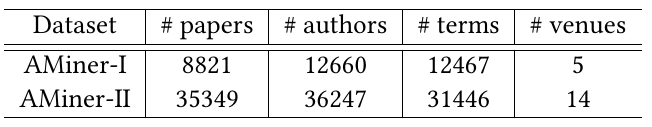
\includegraphics[width=0.8\textwidth]{img/datasets}
% % 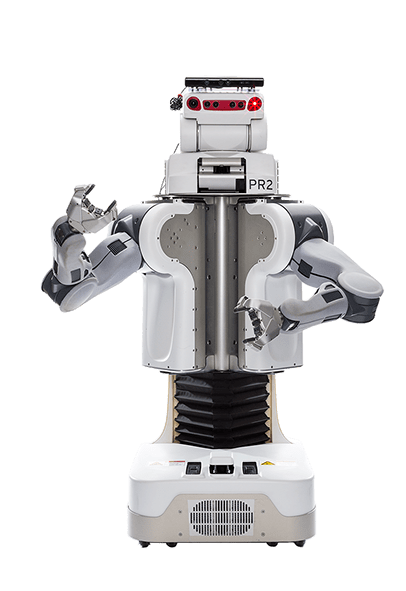
\includegraphics[width=0.8\textwidth]{img/pr2/pr2_a}
% \end{tabular}
% \end{center}
% \end{columns}
\end{frame}
%%%%%%%%%%%%%%%%%%%%%%%%%%%%%%%%%%%%%%%%%%%%%%%%%%%%%%%%%%%%%%%%%%%%%%%%%%%%%%%%%%%%%%%%%%%%%%%%%%%%%%%%%%%%%%%%%%%%%%%%